\documentclass[a4paper, 11pt]{report}
\usepackage[left=2cm, right=2cm, top=1.2cm, bottom=2cm]{geometry}
\usepackage{amsmath,amssymb}
\usepackage{graphicx}
\usepackage{authblk}
%\setlength{\columnsep}{0.8cm}
\usepackage[colorlinks=true,linkcolor=black,urlcolor=blue,filecolor=blue,citecolor=blue]{hyperref}
\usepackage{url}
%\usepackage{CJKutf8} %Only for PDFLaTeX

%%% Only for XeLatex %%%
\usepackage{fontspec} %加這個就可以設定字體
\usepackage{xeCJK} %讓中英文字體分開設置
\setCJKmainfont{標楷體} %設定中文的字型,可以直接輸入系統裡有的字型
\XeTeXlinebreaklocale "zh"
\XeTeXlinebreakskip = 0pt plus 1pt %上面這二行,中文才能自動換行

\title{\textbf{建模報告}}
\author{鄭詠澤\and 陳郁錡\and 游家竣\and 梁恩齊}
\date{\today}

\begin{document}
\maketitle
\tableofcontents

\chapter{問題解析}

\section{題目敘述}

$\quad$在課堂中我們提到一線道公路上的交通流模型。我們首先針對一線道交通流進行速度函數的設定。\\

假設車流密度為 $\rho$,請設定出一個速度函數 V ($\rho$) 滿足下面要求:
公路上速度上限為 A,速度下限 B。在此 A > B,且除了塞車的狀況駕駛人皆不會違規。\\

假設現在有兩線道,其上的車流密度分別為 $\rho 1$ 與 $\rho 2$,此兩函數皆為 x 與 t 的函數。進一步假設:

\begin{itemize}
\item[1.] 兩車道上的駕駛人駕駛習慣一致(皆由一線道交通流所給定的速度函數來行駛)。

\item[2.] 兩車道的速度差 C 以上時有固定比率的車會換道行駛(由速度慢往速度快的車道移動)。
 
\item[3.] 只有公路的起點允許車輛進入公路,公路的終點允許車輛離開公路。
\end{itemize}

試著給定不同的初始條件與邊界條件(以及數值 A, B, C)進行模擬,觀察是否出現所謂的塞車現象(部份路段時速低於 B)。

\chapter{研究與解題方向}
\section{單線道問題}

$\quad$我們參考了幾份文件\cite{Lighthill}\cite{traffic2016research}\cite{model},把離散的車流利用連續流體模型去模擬,並採用一維守恆率:\\

$\frac{\partial}{\partial t} \rho(x, t) + \frac{\partial}{\partial x} Q(x, t) = q(x, t)$\\

由於題目假設只有公路的起點允許車輛進入,終點允許車輛離開,因此進出的車輛是相等的,所以 $q(x,t) = 0$。 遇到連續的狀況,守恆式可寫成:

\begin{equation}
\frac{\partial Q}{\partial x}+\frac{\partial \rho}{\partial t}=0
\end{equation}

加入 $Q = f(\rho)$,令 $\frac{dQ(\rho)}{dk} = c(k)$,則上式可改寫為:

\begin{equation}
\because \frac{\partial Q}{\partial x}=\frac{dQ}{d\rho}\frac{\partial \rho}{\partial x} = c(\rho)\frac{\partial \rho}{\partial x}
\end{equation}

\begin{equation}
\therefore \frac{\partial Q}{\partial x}+\frac{\partial \rho}{\partial t}=c(\rho)\rho_x+\rho_t = 0
\end{equation}

一般稱$c(\rho)$為 traffic wave ,代表穩定車流些微擾動的傳遞(方向與速度)。式 (2.3) 偏微分式待解的未知數只剩一個狀態變數 $\rho$ (代表車流狀態,例如 $\rho = \rho_j$ 代表壅塞),稱為一階準線性偏微分公式(first order quasi-linear partial
differential equation),可以特性根法 (characteristics method) 解析求解。\\

式 (2.3) 簡單連續流模式的解析解 (analytical solution)。 如觀察密度的變化,其數學式可寫成:

\begin{equation}
d\rho = \frac{\partial \rho}{\partial t}dt+\frac{\partial \rho}{\partial x}dx⇒\frac{d\rho}{dt}=\rho_t+\rho_x\frac{dx}{dt}
\end{equation}

\begin{equation}
\frac{d\rho}{dt} = \rho_t+\rho_x\frac{dx}{dt}=\rho_t+c(\rho)\rho_x
\end{equation}

由式 (2.3) 可知,式 (2.5) 等於 0,亦即隨車波前進,觀察到的密度根本沒有改變。依數學定義,車波 $c = \frac{dq}{d\rho}$ 是流率-密度曲線上某點的切線,單位為速率(公里/小時)。由以上的分析知,因為沿車波前進,車密度不變,因此車波線可代表某車流狀態由邊界條件發散出來後在時空上的直線擴散或運動,相對的,車波線只要維持直線,即代表車流狀態(密度)維持不變。\\

我們需要知道整條路 $x \in [0, L_{road}]$ 在一開始($t = 0$) 的 initial condition $\rho(x,0)$。在沒有塞車的情況下,$\rho(0,t) < \rho_c$,流速的上界(BC) $\rho(0,t) = \rho_{free}(Q_{up}(t))$ 由每條路的 traffic demand $Q_{up}$ 來控制。 而在塞車的情況下,下界 $\rho(L_{road},t) = \rho_{cong}(Q_{down}(t))$ 由塞車時能承受的最大流量來決定。

\newpage
\section{差分法}

\begin{itemize}
\item Explicit 數值方法: 只需要前後數值
\item First-order 方法: 如果 $\Delta t$ 和 $\Delta x$ 都趨近於零,則時間間隔內的誤差會隨著 t 和 x 線性減少
\item Euler method: 對所有的 $f(t)$,$f(t+\Delta t) \approx f(t) + f'(t)$

如果沒有塞車,則
\begin{equation*}
\rho_{k,j+1} = \rho_{k,j} - \frac{\Delta t}{\Delta x}(Q_{k-1,j} - Q_{k,j})
\end{equation*}
\begin{equation*}
Q_{k,j+1} = Q_e(\rho_{k,j+1})
\end{equation*}

如果塞車,則
\begin{equation*}
\rho_{k,j+1} = \rho_{k,j} - \frac{\Delta t}{\Delta x}(Q_{k+1,j} - Q_{k,j})
\end{equation*}
\begin{equation*}
Q_{k,j+1} = Q_e(\rho_{k,j+1})
\end{equation*}

\end{itemize}

\section{模型選定}

我們直接選用 greensheilds 模型,車子 (平均) 速度 𝑣 與車流密度 𝑘 呈現線性關係: $v = v_f (1- \frac{\rho^2}{\rho_j}$,流量與密度的函數關係式:$q = v_f(\rho-\frac{\rho^2}{\rho_j})$,流量與速度的函數關係式:$q = \rho_j(v-\frac{v^2}{v_Q})$
\begin{figure}[htbp]
\centerline{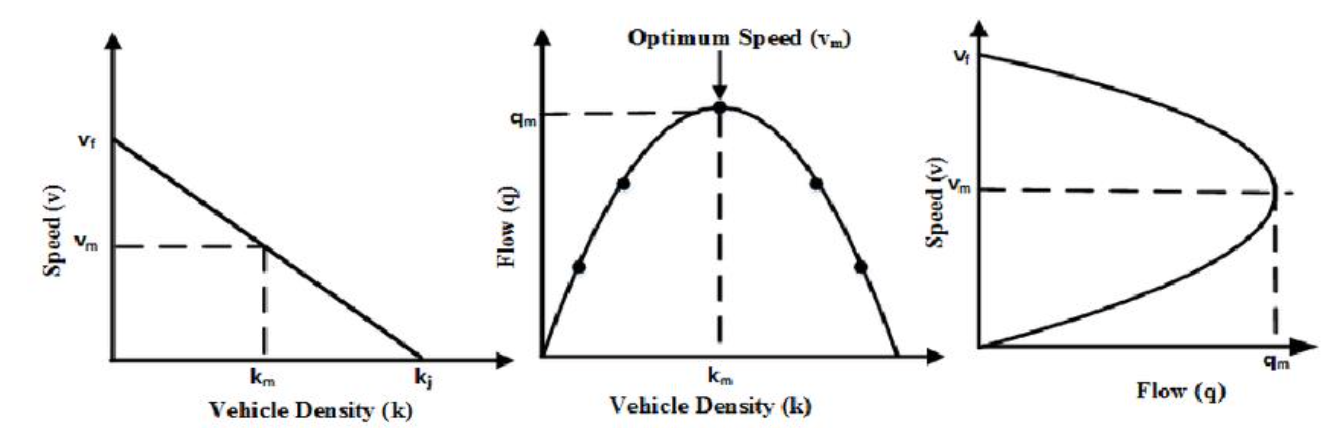
\includegraphics[height=2in]{function.png}}
\caption{函數關係圖}
\label{program_flowchart}
\end{figure}

但結果不太理想,所以後來我們還用了中央差分法,加上 ODE45,,設定了一些比較好的邊界條件,可以看出裡面的塞車回堵狀況,模擬出了一個新的圖。

\begin{figure}[htbp]
\centerline{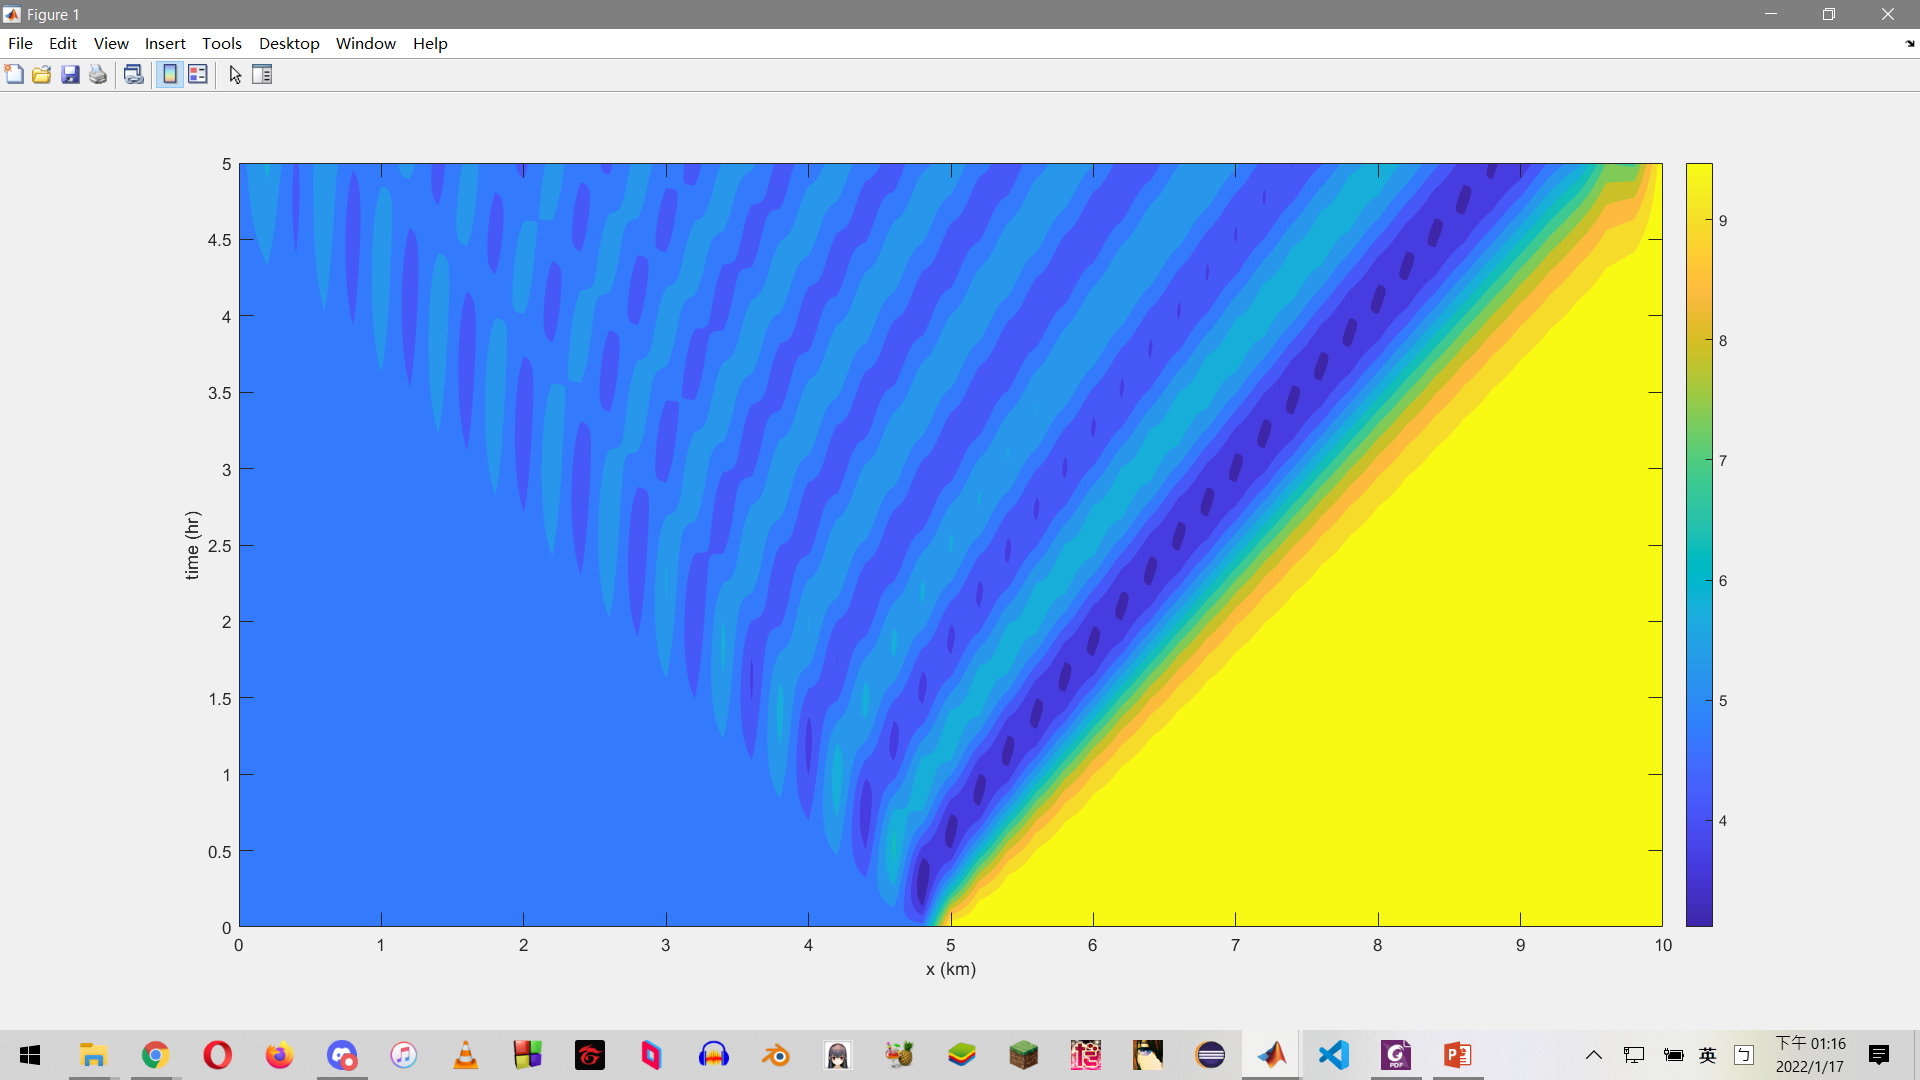
\includegraphics[height=2in]{output1.png}}
\caption{ODE 差分圖}
\label{program_flowchart}
\end{figure}

\newpage

但若用實際資料去跑,結果與預期的差很多,圖像這樣:
\begin{figure}[htbp]
\centerline{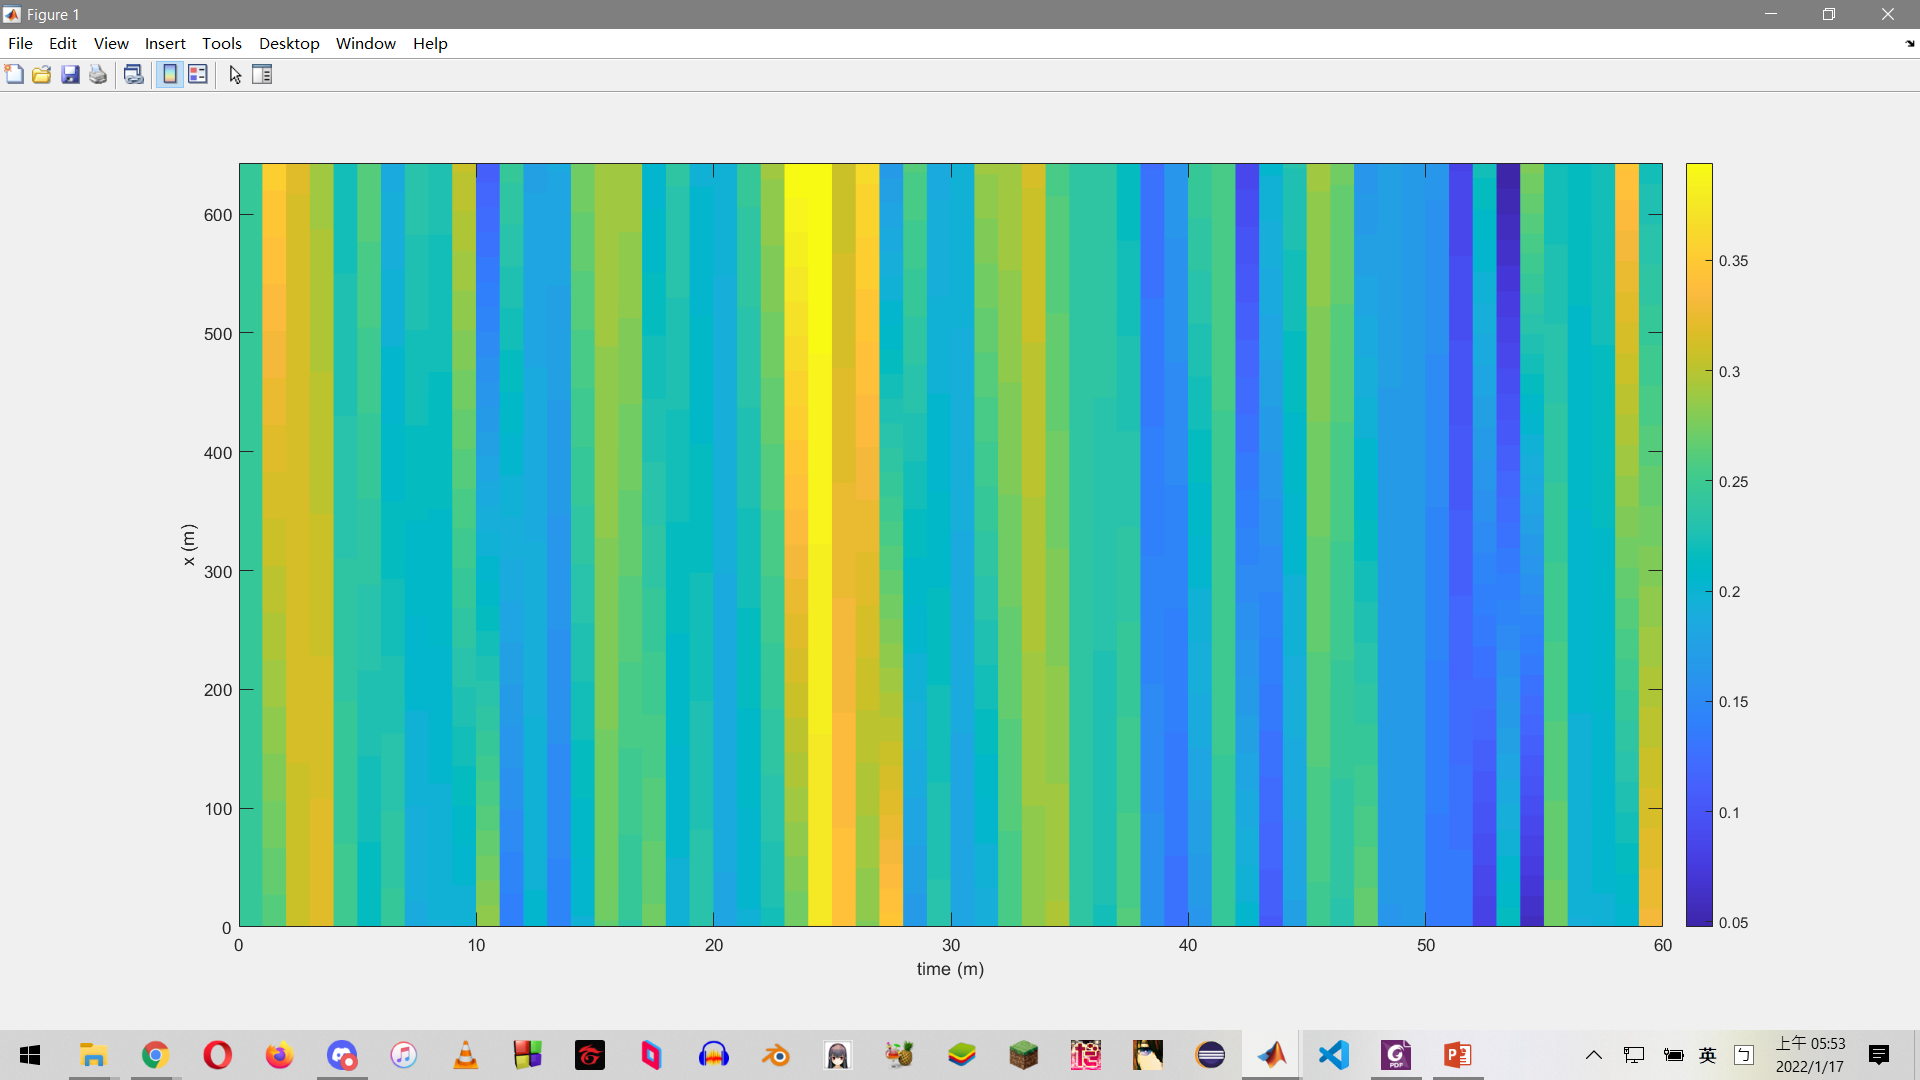
\includegraphics[height=2in]{real.png}}
\caption{實際資料模擬圖}
\label{program_flowchart}
\end{figure}

greensheild 裡面有兩個係數,因為是跟 V 的關係式,所以給定 N 筆資料,就可以寫出一個係數矩陣,就可以用最小平方法把 $V_f(\rho_j)$ 算出來。 然後測站之間去做差值,如果有更多連續的測站,就可以減少差值去看整個路段,會更接近真實的解。

\section{結論}

$\quad$我們在用差分的過程中用了兩種方法,一種是本差分法,令一種是中央差分+ODE45,兩個方法都明顯有問題,原因是初始值沒辦法給的很連續,改善的方法是在取資料時要取密度高一點的感測器資料,越密越連續,但由於時間緊迫,我們現在尚未完成。

如果我們能改善這個問題,就可以解決單線道的車流問題了,再用雙車道的資料於 ODE45 裡面寫判斷式,判斷換車道問題,就可以解決雙車道的轉換問題。

\renewcommand{\bibname}{References}
\bibliographystyle{plain}
\bibliography{final}
\end{document}